\documentclass{article}
\usepackage[usenames, dvipsnames]{color}
\usepackage{graphicx}
\usepackage{caption}
\usepackage{subcaption}
\usepackage{hyperref}
\usepackage{longtable}
\usepackage{float}
\hypersetup{
	citecolor=black,
	filecolor=black,
	linkcolor=black,
	urlcolor=black
}
\graphicspath{ {images/} }

\title{Dynamic sampling pointnet notes}
\author{xyz}
\date{Feb 2018}

\begin{document}
\begin{titlepage}
\maketitle
\end{titlepage}	

\tableofcontents{}

\section{Quick notes for important events while using one file to test}
\subsection{batch size}
\subsubsection{bs=27 vs bs=81}
batch size: 9,27,81 \par
data: xyz-color\_1norm\par
model: 1AG\par
sampling \& grouping: stride\_0d1\_step\_0d1\_bmap\_nh5\_2048\_0d5\_1\_fmn1-160\_32-32\_12-0d2\_0d6-0d2\_0d6\par
\begin{figure}[h!]
	\caption{bs=9}
	\centering
	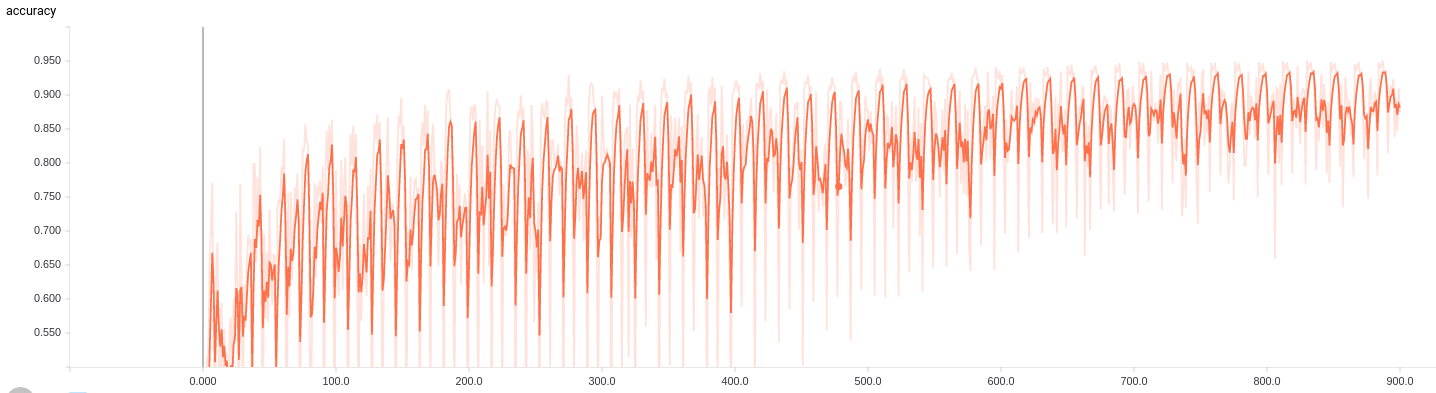
\includegraphics[width=\textwidth]{acc_log-model_1AG-gsbb_2C1-bs9-xyz-color_1norm-2048-mat}
	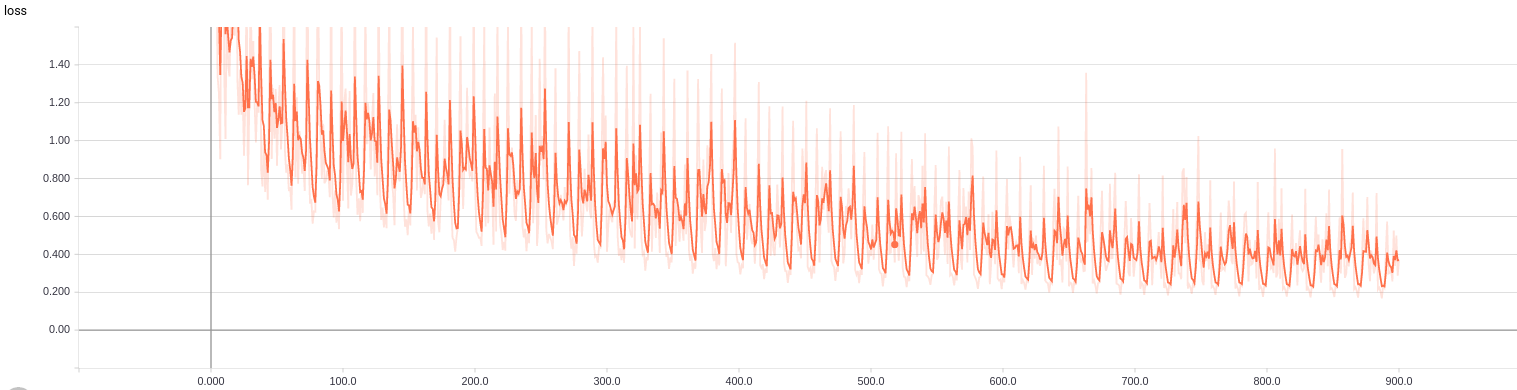
\includegraphics[width=\textwidth]{loss_log-model_1AG-gsbb_2C1-bs9-xyz-color_1norm-2048-mat}
\end{figure}
\begin{figure}[h!]
	\caption{bs=27}
	\centering
	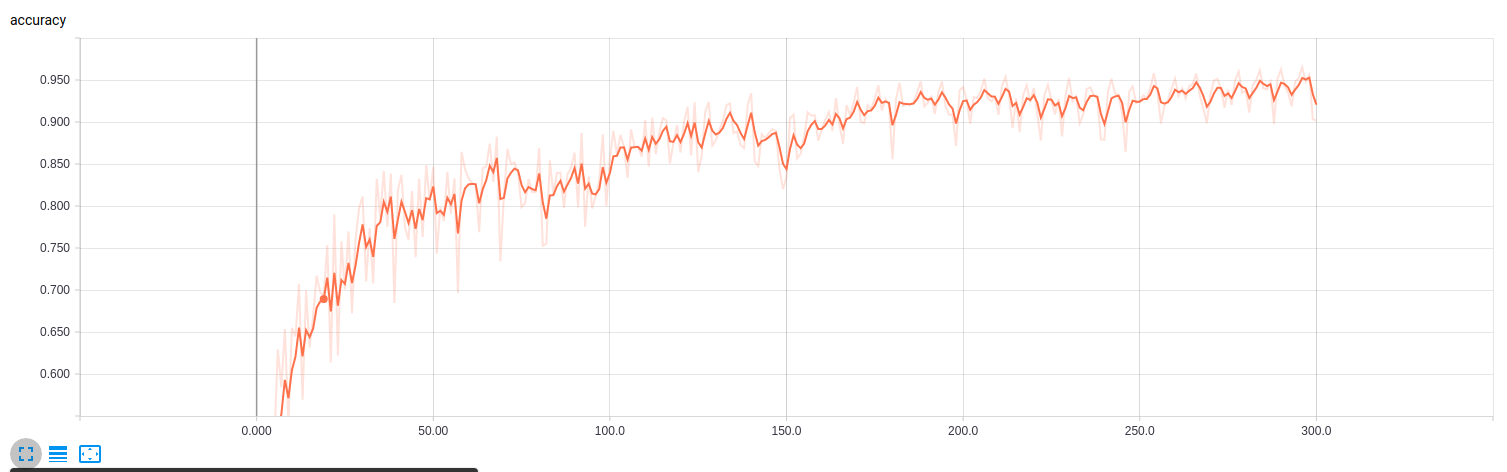
\includegraphics[width=\textwidth]{acc_log-model_1AG-gsbb_2C1-bs27-xyz-color_1norm-2048-mat}
	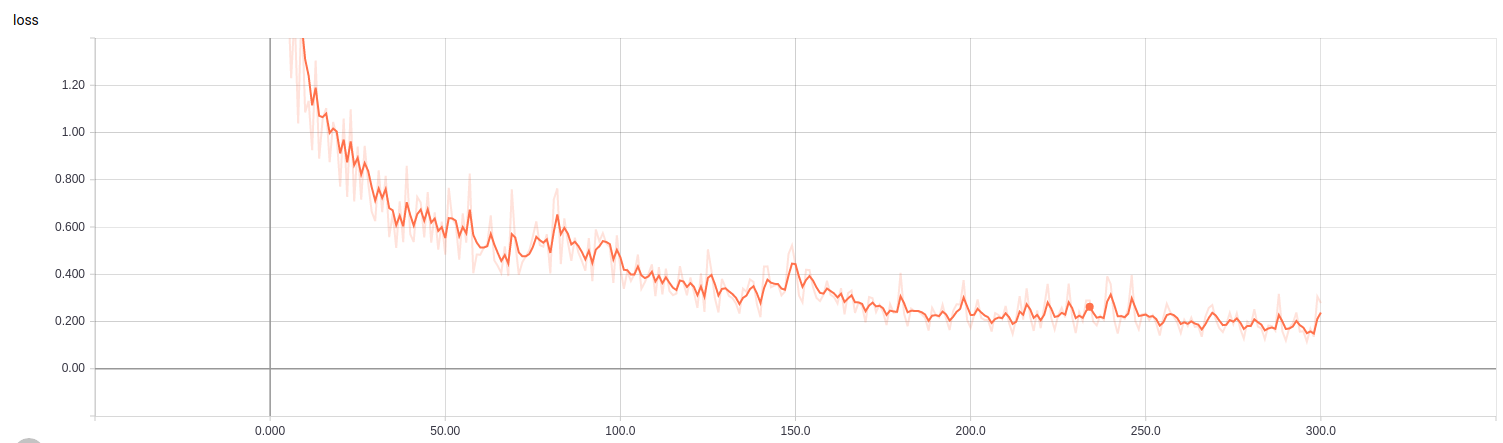
\includegraphics[width=\textwidth]{loss_log-model_1AG-gsbb_2C1-bs27-xyz-color_1norm-2048-mat}
\end{figure}
\begin{figure}[h!]
	\centering
	\caption{bs=81}
	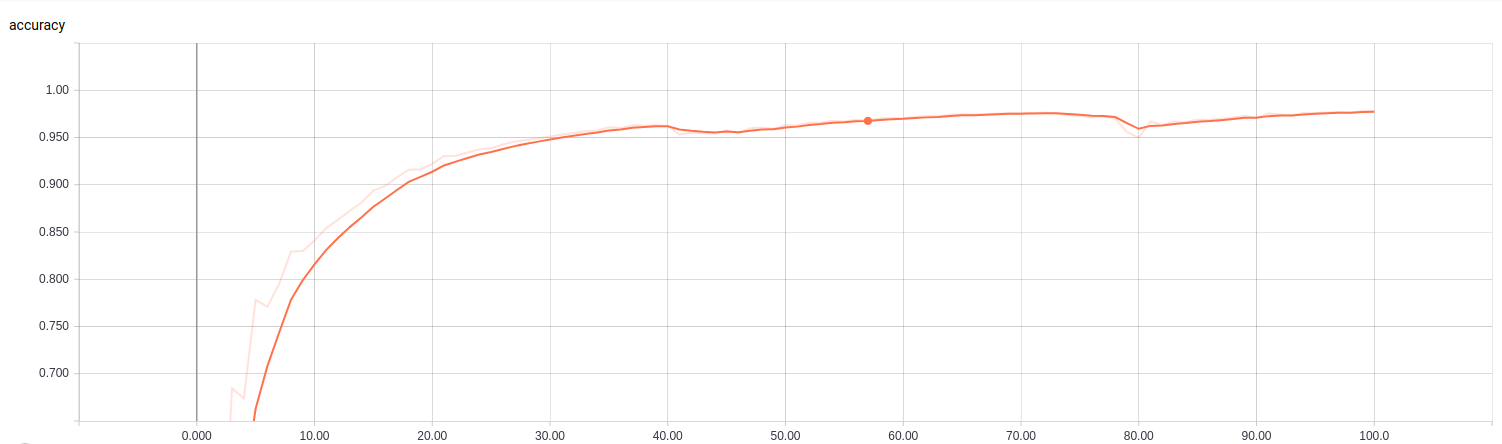
\includegraphics[width=\textwidth]{acc_log-model_1AG-gsbb_2C1-bs81-xyz-color_1norm-2048-mat}
	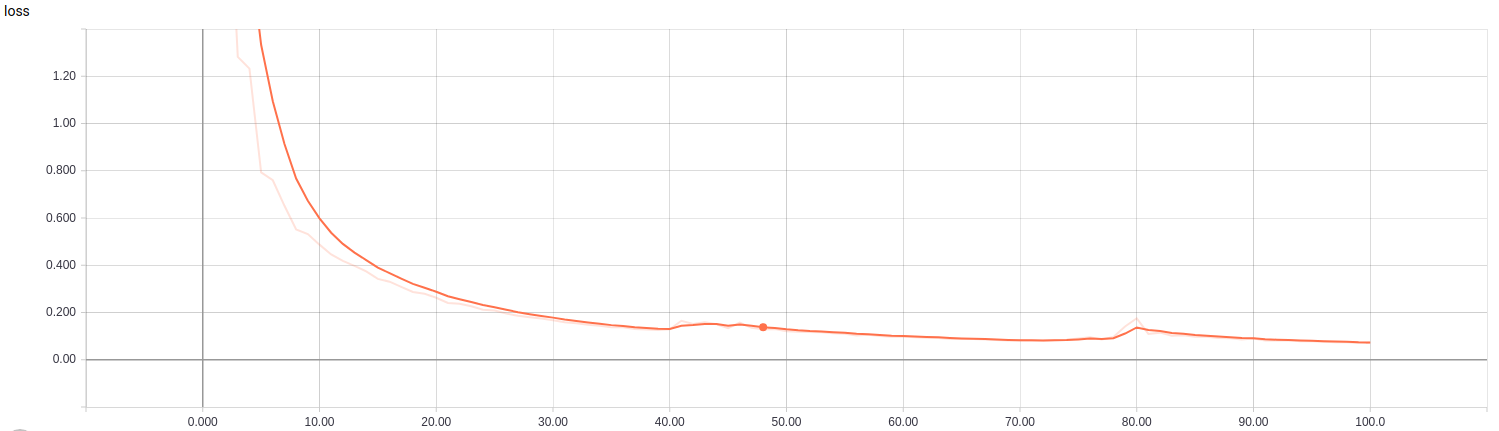
\includegraphics[width=\textwidth]{loss_log-model_1AG-gsbb_2C1-bs81-xyz-color_1norm-2048-mat}
\end{figure}

\subsection{feed elements}
epoch num = 100 \par
stride\_0d1\_step\_0d1\_bmap\_nh5\_2048\_0d5\_1\_fmn1-160\_32-32\_12-0d2\_0d6-0d2\_0d6 \par
\begin{center}
	\begin{tabular}{|c |c | c || c c |} 
		\hline
		model & batch size & data elements & acc & loss \\
		\hline
		1AG & 9 & xyz color & 0.890 & 0.356\\ [0.5ex] 
		\hline
		1AG & 27 & xyz color & 0.920 & 0.240\\ [0.5ex] 
		\hline
		
		3AG & 27 & xyz color& 0.912 & 0.273 \\  [0.5ex]
		\hline
		2A & 27 & xyz color& 0.908 & 0.294 \\  [0.5ex]
		\hline
		2AG & 27 & xyz color& 0.902 & 0.293 \\  [0.5ex]
		\hline
		1A & 27 & xyz color& 0.883 & 0.351 \\  [0.5ex]
		\hline
		1AG & 81 & xyz color & 0.978 & 0.072\\ [0.5ex] 
		\hline\hline
		
		1AG & 9 & xyz  & 0.861 & 0.427\\ [0.5ex] 
		\hline
		1AG & 27 & xyz & 0.907 & 0.257\\ [0.5ex] 
		\hline
		1AG & 81 & xyz & 0.975 & 0.078 \\  [0.5ex]
		\hline\hline
		1A & 27 & xyzmid color& 0.889 & 0.357 \\  [0.5ex]
		\hline
		3AG & 27 & xyzmid color& 0.933 & 0.193 \\  [0.5ex]
		\hline
		
		2A & 27 & xyzmid color& 0.939 & 0.177 \\  [0.5ex]
		\hline
		
		2AG & 27 & xyzmid color& 0.929 & 0.208 \\  [0.5ex]
		\hline\hline
		3AG & 27 & xyz xyzmid color& 0.924 & 0.230 \\  [0.5ex]
		\hline
		
		2A & 27 & xyz xyzmid color& 0.898 & 0.317 \\  [0.5ex]
		\hline
		2AG & 27 & xyz xyzmid color& 0.908 & 0.280 \\  [0.5ex]
		\hline
		1A & 27 & xyz xyzmid color& 0.910 & 0.281 \\  [0.5ex]
		\hline
		1AG & 27 & xyz xyzmid color& 0.944 & 0.163 \\  [0.5ex]
		\hline
		1AG & 81 & xyz xyzmid color& 0.976 & 0.078 \\  [0.5ex]
		\hline
		2A & 81 & xyz xyzmid color& 0.942 & 0.173 \\  [0.5ex]
		\hline
		3AG & 81 & xyz xyzmid color& 0.949 & 0.147 \\  [0.5ex]
		\hline
	\end{tabular}
\end{center}

1. large batch size is better \par
2. $1AG (0.92) > 3AG(0.912) > 2A(0.908) > 2AG(0.902) > 1A(883)$ \par
   1AG is much better than 1A \par 
   \textbf{1AG is a bit better than 3AG ???} \par

3. xyz-color is only a bit better than xyz \par
4. xyzmid-color is much better than xyz-color \par
5. \textbf{xyzmid-color is normally much better than xyz-xyzmid-color ???} \par



\subsection{model}
batch size: 50 \par
data: xyz\_midnorm\_block-color\_1norm \par
epoch\_num = 600 \par
sampling \& grouping: stride\_0d1\_step\_0d1\_bmap\_nh5\_12800\_1d6\_2\_fmn3-600\_64\_24-60\_16\_12-0d2\_0d6\_1d2-0d2\_0d6\_1d2 \par
\begin{center}
	\begin{tabular}{|c | c c |} 
		\hline
		model  & acc & loss \\
		\hline
		3A & 0.909 & 0.248 \\ [0.5ex] 
		\hline
		3AG & 0.913 & 0.231 \\ [0.5ex] 
		\hline
		4AG & 0.912 & 0.232 \\ [0.5ex] 
		\hline	
	\end{tabular}
\end{center}

batch size: 32 \par
data: xyz\_midnorm\_block-color\_1norm \par
sampling \& grouping: stride\_0d1\_step\_0d1\_bmap\_nh5\_12800\_1d6\_2\_fmn6-2048\_256\_64-32\_32\_16-0d2\_0d6\_1d2-0d1\_0d3\_0d6 \par
matterport3d  \par
feed\_data\_elements:['xyz\_midnorm\_block', 'color\_1norm']  \par
feed\_label\_elements:['label\_category', 'label\_instance']  \par
train data shape: [  362 12800     6]  \par  
test data shape: [  384 12800     6] \par
max epoch = 500
\begin{center}
	\begin{tabular}{|c | c c |} 
		\hline
		model  & acc & loss \\
		\hline
		1AG & 0.944/0.431 & 0.161/4.633 \\ [0.5ex] 
		\hline
		
		4AG & 0.835/0.401 & 0.520/3.644 \\ [0.5ex] 
		\hline	
	\end{tabular}
\end{center}

\subsection{integration: matterport3d}
\begin{center}
	\centering \def\arraystretch{1.5} \small
	\begin{longtable}{|p{1cm} |p{1.5cm} | p{2cm} | p{3.5cm} || p{4cm}|} 
		\hline
		\multicolumn{5}{|c|}{stride\_0d1\_step\_0d1\_bmap\_nh5\_12800\_1d6\_2\_fmn3-512\_64\_24-48\_16\_12-0d2\_0d6\_1d2-0d2\_0d6\_1d2 }\\
		\multicolumn{5}{|c|}{17D\_1LX\_1pX\_29h\_2az}\\
		\hline
		model & batch size\par batch num \par shuffle& lr\par ds & data elements & epoch-acc mean-std \par train/eval \\
		\hline
		1aG & 30/60 & 0.005 & 'xyz\_midnorm\_block', 'color\_1norm', 'nxnynz'& 250-0.981  \\  [0.5ex]
		\hline
		1DSaG & 30/60 & 0.001-40 & 'xyz\_midnorm\_block', 'color\_1norm', 'nxnynz'& 300-0.914-0.775  \\  \hline
		1DSaG & 30/60 & 0.001-40 & 'xyz\_midnorm\_block', 'color\_1norm', 'nxnynz'& 300-0.914-0.775  \\  [0.5ex] \hline
		1DSaG \par kp0.5& 30/60 & 0.001-80\par 300-3e-4 & 'xyz\_midnorm\_block', 'color\_1norm', 'nxnynz'& 300-0.942-0.842  \\  [0.5ex] \hline
		1DSaG \par kp0.2& 30/60 & 0.001-80\par 300-3e-4 & 'xyz\_midnorm\_block', 'color\_1norm', 'nxnynz'& 300-0.928-0.797  \\  [0.5ex] \hline
		1DSaG \par kp0.5& 30/60 & 0.005-80\par 300-1.7e-3 & 'xyz\_midnorm\_block', 'color\_1norm', 'nxnynz'& 300-0.970-0.916  \\  [0.5ex] \hline
		1DSaG \par kp0.2& 30/60 & 0.005-80\par 300-1.7e-3 & 'xyz\_midnorm\_block', 'color\_1norm', 'nxnynz'& 300-0.966-0.924  \\  [0.5ex] \hline
		1DSaG \par kp0.8& 30/60 & 0.005-80\par 300-1.7e-3 & 'xyz\_midnorm\_block', 'color\_1norm', 'nxnynz'& 300-0.976-0.933 \par 500-0.984-0.954 \\  [0.5ex] \hline
		
		
		\hline\hline
		1aG & 30/1083 & 0.003 & 'xyz\_midnorm\_block', 'color\_1norm', 'nxnynz'& 200-0.947  \\  [0.5ex]
		\hline		
		1aG & 30/1083 & 0.01  & 'xyz\_midnorm\_block', 'color\_1norm'& 200-0.783 \par 500-0.791  \\  [0.5ex]
		\hline		
		1aG & 30/1083 & 0.003/30 \par 300-0.00012 & 'xyz\_midnorm\_block', 'color\_1norm'& 200-0.903 \par 300-0.921  \\  [0.5ex]
		\hline\hline
		
		1bG & 25/1083 & 0.001-30 \par 100-3e-4 \par 300-4e-5 & 'xyz\_midnorm\_block'& 100-0.854 \par 200-0.918 \par 300-0.936  \\  [0.5ex]
		\hline
		1bG & 25/1083 & 0.001-30 \par 100-3e-4 \par 300-4e-5 & 'xyz\_midnorm\_block', 'color\_1norm', 'nxnynz'& 100-0.914 \par 200-0.957 \par 300-0.966  \\  [0.5ex]
		\hline	
		1bG & 25/1083 & 0.02 & 'xyz\_midnorm\_block', 'color\_1norm'& 200-0.655 \par 300-0.718  \\  [0.5ex]
		\hline
		1bG & 25/1083 & 0.02 & 'xyz\_midnorm\_block', 'color\_1norm', 'nxnynz'& 200-0.772 \par 300-0.823  \\  [0.5ex]
		\hline
		1bG & 25/1083 & 0.001 & 'xyz'& 200-0.772 \par 90-0.553-0.210  \\  [0.5ex]
		\hline \hline
		
		4bG & 25/1083 & 0.001-30 \par 100-3e-4 \par 200-1e-4 \par 300-4e-5& 'xyz\_midnorm\_block', 'color\_1norm', 'nxnynz'& 100-0.752 \par 200-0.816 \par 300-0.832  \\  [0.5ex] \hline2
		
		1DSaG & 30/1083 & 0.002-80 & 'xyz\_midnorm\_block', 'color\_1norm', 'nxnynz'& 200-0.930-0.830/0.450 \par 460-0.952-0.881/0.471 \\  [0.5ex] \hline
		
		\hline \hline
		1aG & 30/19755 & 0.001-30 \par 50-7e-4 \par 100-3e-4& 'xyz\_midnorm\_block', 'color\_1norm','nxnynz'& 50-0.752/0.580 \par 100-0.843/0.574 (\colorbox{Yellow}{NoShuf}) \par 102-0.806/0.570 (\colorbox{Yellow}{Shufle})   \\  [0.5ex]
		\hline
		1bG & 25/19755 & 0.001-30& 'xyz\_midnorm\_block', 'color\_1norm','nxnynz'& 38-0.719/0.587 \par 80-0.823/0.583 (\colorbox{Yellow}{NoShuf}) \par 81-0.782/0.587 (\colorbox{Yellow}{Shufle}) \\  [0.5ex]
		\hline
		1aG & 30/19755 & 0.02 & 'xyz\_midnorm\_block', 'color\_1norm'& 56-0.562   \\  [0.5ex]
		\hline
		1aG & 30/19755 & 0.02 \par 127-0.00483& 'xyz\_midnorm\_block', 'color\_1norm', 'nxnynz'& 87-0.616 \par 127-0.686 \\  [0.5ex]
		\hline
		\hline
		1bG & 25/18737 & 0.001 \par N& 'xyz\_midnorm\_block', 'color\_1norm', 'nxnynz'& 24-0.682/0.509 \par 70-0.858/0.509\\  [0.5ex]
		\hline
		1bG & 25/18737 & 0.001 \par Y& 'xyz\_midnorm\_block', 'color\_1norm', 'nxnynz'& 24-0.738/0.573 \par 70-0.876/0.563 \par \colorbox{Yellow}{90-0.897}/0.561\\  [0.5ex]
		\hline
		4bG & 25/18737 & 0.001 \par Y& 'xyz\_midnorm\_block', 'nxnynz'& 24-0.576/0.545 \\  [0.5ex]
		\hline
		4bG & 25/18737 & 0.001 \par Y& 'xyz\_midnorm\_block', 'color\_1norm', 'nxnynz'& 24-0.594/0.569 \\  [0.5ex]
		\hline
		1DSaG & 30/18737 & 0.002-80 \par Y& 'xyz\_midnorm\_block', 'color\_1norm', 'nxnynz'& 20-0.688-0.394/0.428-0.224 \par 36-0.742/0.395 \\  [0.5ex]
		\hline
		1DSaG & 30/18737 & 0.007-80 \par Y& 'xyz\_midnorm\_block', 'color\_1norm', 'nxnynz'& 20-0.725-0.453/0.435-0.206 \par 38-0.783/0.396 \\  [0.5ex]
		\hline
		\multicolumn{5}{|l|}{ \shortstack[l]{Conclusion:\\ 
				1: nxnynz helps a lot \\
				2: 1bG is much deeper than 1aG, why worse than 1aG \\
				3: learning rate is important, cannot be too large
		} }  \\
		\hline
	\end{longtable}
\end{center}

\subsection{integration: scannet}
\begin{center}
	\centering \def\arraystretch{1.5} \small
	\begin{tabular}{|p{1cm} |p{1cm} |p{1.5cm} | p{2cm} | p{2cm} || p{5cm}|} 
		\hline
		\multicolumn{6}{|c|}{stride\_0d1\_step\_0d1\_bmap\_nh5\_12800\_1d6\_2\_fmn3-256\_48\_16-56\_8\_8-0d2\_0d6\_1d2-0d2\_0d6\_1d2 }\\
		\multicolumn{6}{|c|}{ scannet train }\\
		\hline
		model & loss: E,N,C \par input drop (No) & batch size\par batch num \par shuffle& lr\par ds & data elements & epoch-point ac-class ac \par train/eval \\
		\hline
		1bG & E & 25/12887\par test \par Y & 0.001\par 40 & xyzmid & 23-0.732-0.326/0.664-0.260 \par 25-0.746-0.340/0.669-0.273\\ \hline
		1bG & N & 25/12887\par Y & 0.001\par 40 & xyzmid & 25-0.733-0.390/0.666-0.252\\ \hline
		1bG & C & 25/12887\par Y & 0.001\par 40 & xyzmid & 25-0.703-0.356/0.655-0.252\\ \hline
		1bG & CN & 25/12887\par Y & 0.001\par 40 & xyzmid & 25-0.681-0.366/0.611-0.237\\ \hline
		1DSaG & E \par idp9& 30/12887\par Y & 0.003\par 80 & xyzmid & 40-0.738-0.376/\colorbox{yellow}{0.513}-0.228\\ \hline
		
		\hline\hline
		1bG & E & 25/13091\par train\_300\par Y & 0.002\par 80 & xyzmid & 60-0.765-0.389/0.700-0.252\\ \hline
		1bG & E & 25/13091\par Y & 0.003\par 80 & xyzmid & 10-0.646/0.689 \par 60-0.753-0.349/0.691-0.234 \par  100-0.833-0.480/0.672-0.261\\ \hline
		1bG & CN & 25/13091\par Y & 0.002\par 80 & xyzmid & 60-0.738-0.409/0.670-0.237\\ \hline
		1bG & E \par idp9 & 25/13091\par Y & 0.003\par 80 & xyzmid & 10-0.641/0.585 \par 16-0.646/0.633\\ \hline
		1DSaG & E & 30/13091\par Y & 0.003\par 80 & xyzmid & 40-0.794-0.456/0.420-0.154 \par 100-0.872-0.602/0.417-0.153\\ \hline
		
		\multicolumn{6}{|p{12.5cm}|}{ Conclusion:\par		 }  \\
		
		\hline\hline
		4bG & CN & 25/2998-3521\par Y & 0.001\par 40 & xyzmid & 142-0.726-0.445/0.625-0.242\\
		\hline
		4bG & E & 25/2998-3521\par Y & 0.001\par 40 & xyzmid & 145-0.792-0.506/0.656-0.257\\
		\hline
	\end{tabular}
\end{center}


\subsection{Semantic segmentation expamples}
\subsubsection{good: 1083, train, 0.946}
log: log-model\_1bG-gsbb\_3B1-bs25-lr1-ds\_30-xyz\_midnorm\_block-color\_1norm-nxnynz-12800-mat\_1083 \par
model: 1bG \par
sampling \& grouping: \par stride\_0d1\_step\_0d1\_bmap\_nh5\_12800\_1d6\_2\_fmn3-512\_64\_24-48\_16\_12-0d2\_0d6\_1d2-0d2\_0d6\_1d2 \par
batch size: 25 \par
learning rate: 0.001000 \par
decay\_epoch\_step: 30 \par
matterport3d  \par
feed\_data\_elements:['xyz\_midnorm\_block', 'color\_1norm', 'nxnynz']  \par
feed\_label\_elements:['label\_category', 'label\_instance']  \par
train data shape: [ 1083 12800     9] \par

\begin{figure}[H]
	\centering
	\begin{subfigure}[h]{0.49\textwidth}
	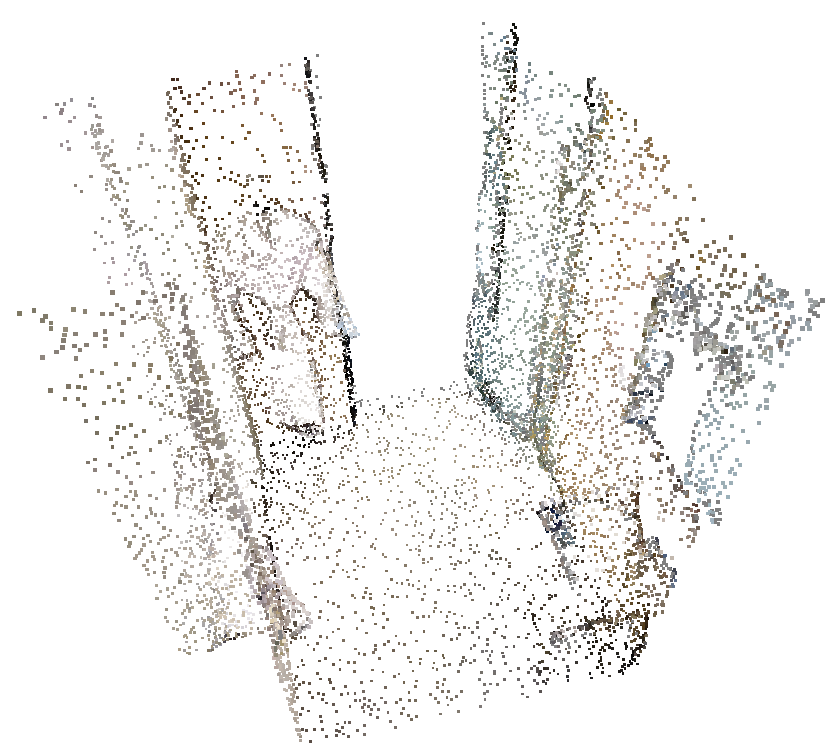
\includegraphics[width=\textwidth]{ply_log-model_1bG-gsbb_3B1-bs25-lr1-ds_30-xyz_midnorm_block-color_1norm-nxnynz-12800-mat_1083/17DRP5sb8fy_1_2_a946/raw00.png}
	\caption{colorized point cloud}
	\end{subfigure}
	\begin{subfigure}[h]{0.49\textwidth}
	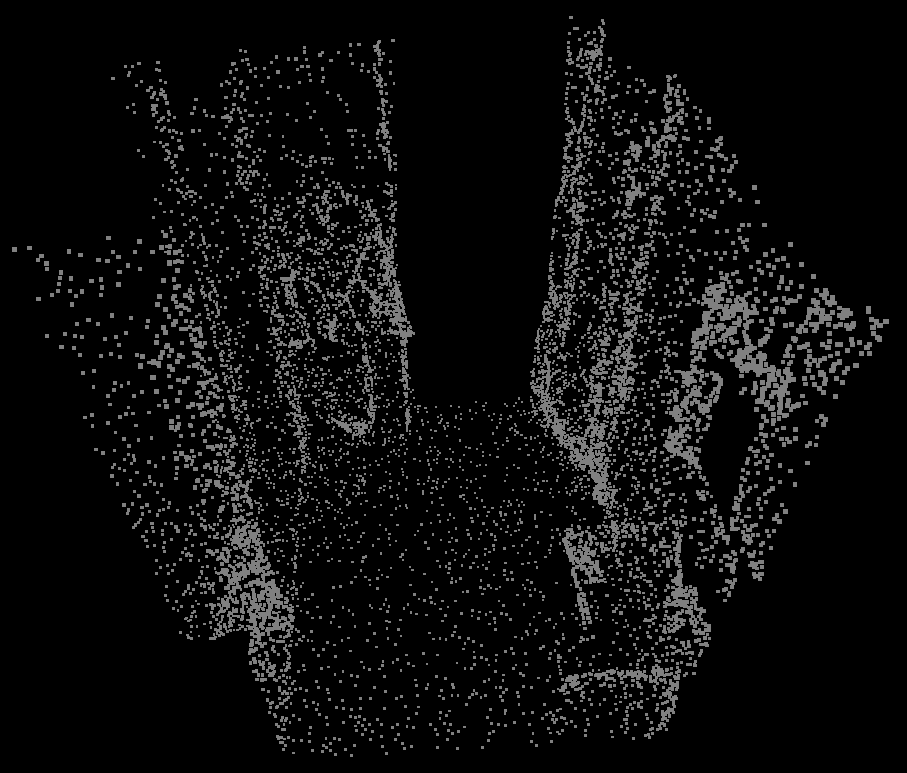
\includegraphics[width=\textwidth]{ply_log-model_1bG-gsbb_3B1-bs25-lr1-ds_30-xyz_midnorm_block-color_1norm-nxnynz-12800-mat_1083/17DRP5sb8fy_1_2_a946/xyz00.png}
	\caption{raw point cloud}
	\end{subfigure}
	\begin{subfigure}[h]{0.5\textwidth}
	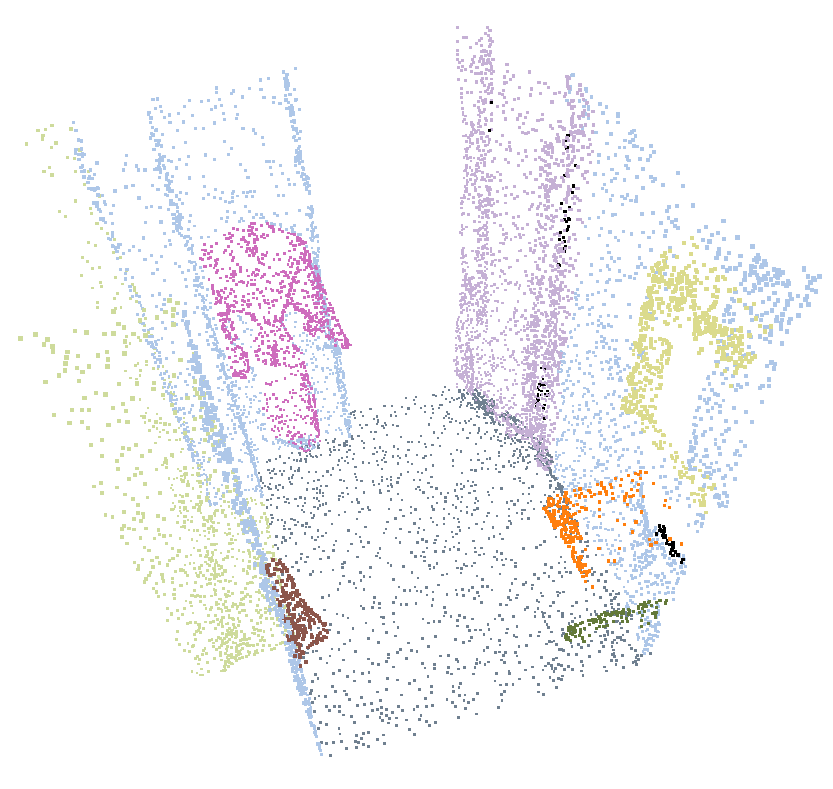
\includegraphics[width=\textwidth]{ply_log-model_1bG-gsbb_3B1-bs25-lr1-ds_30-xyz_midnorm_block-color_1norm-nxnynz-12800-mat_1083/17DRP5sb8fy_1_2_a946/gt00.png}
	\caption{gt}
	\end{subfigure}
	\begin{subfigure}[h]{0.49\textwidth}
	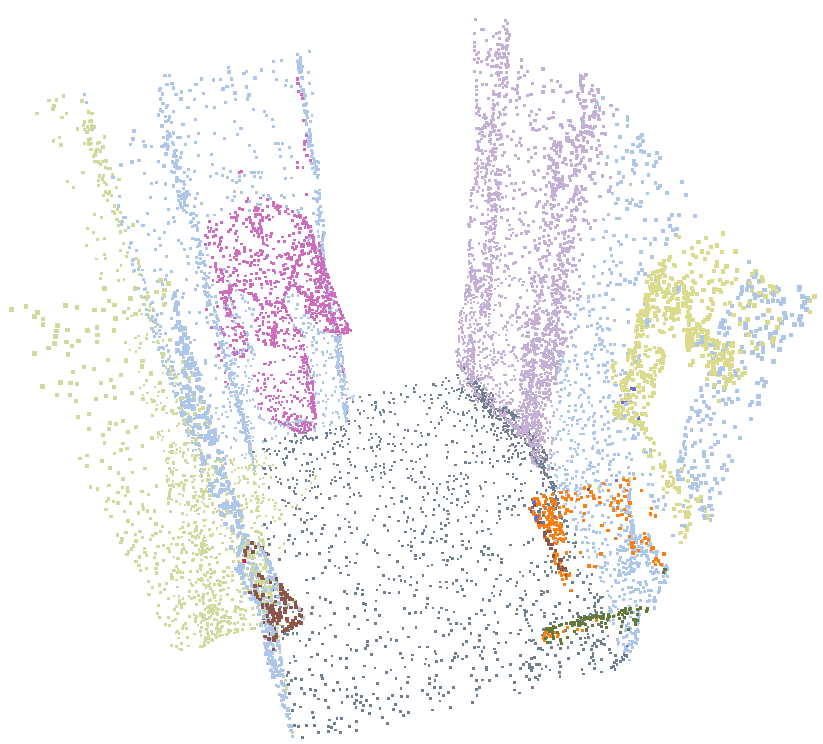
\includegraphics[width=\textwidth]{ply_log-model_1bG-gsbb_3B1-bs25-lr1-ds_30-xyz_midnorm_block-color_1norm-nxnynz-12800-mat_1083/17DRP5sb8fy_1_2_a946/pred00.png}	
	\caption{pred}
	\end{subfigure}
	\begin{subfigure}[h]{0.5\textwidth}
	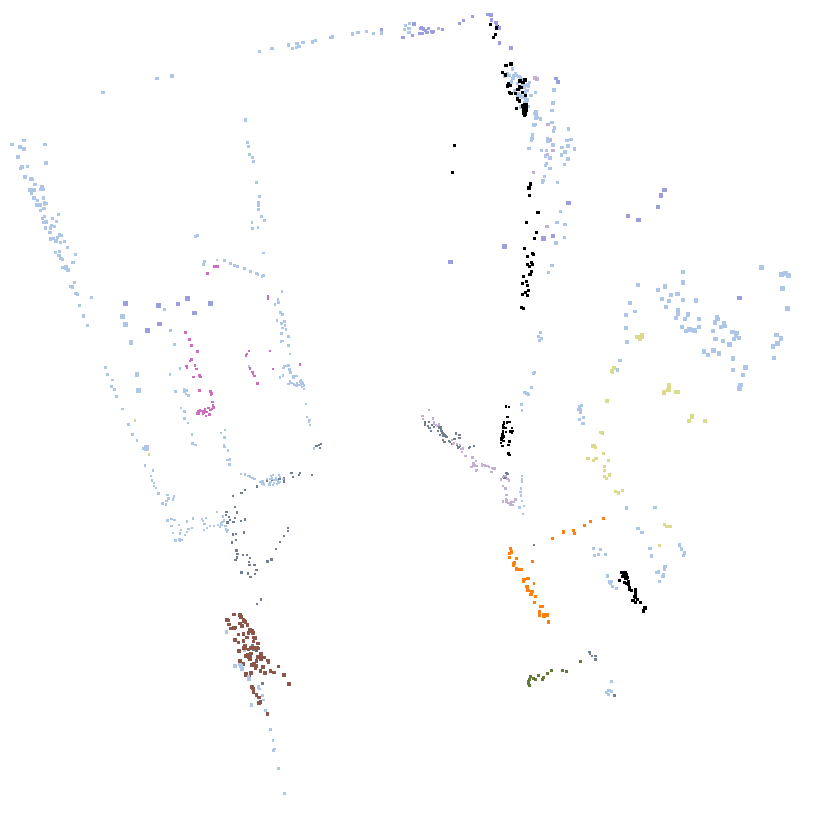
\includegraphics[width=\textwidth]{ply_log-model_1bG-gsbb_3B1-bs25-lr1-ds_30-xyz_midnorm_block-color_1norm-nxnynz-12800-mat_1083/17DRP5sb8fy_1_2_a946/err00.png}
	\caption{err}
\end{subfigure}
	\caption{17DRP5sb8fy\_1\_2\_a946}
\end{figure}

\begin{figure}[H]
	\centering
	\begin{subfigure}[h]{0.5\textwidth}
	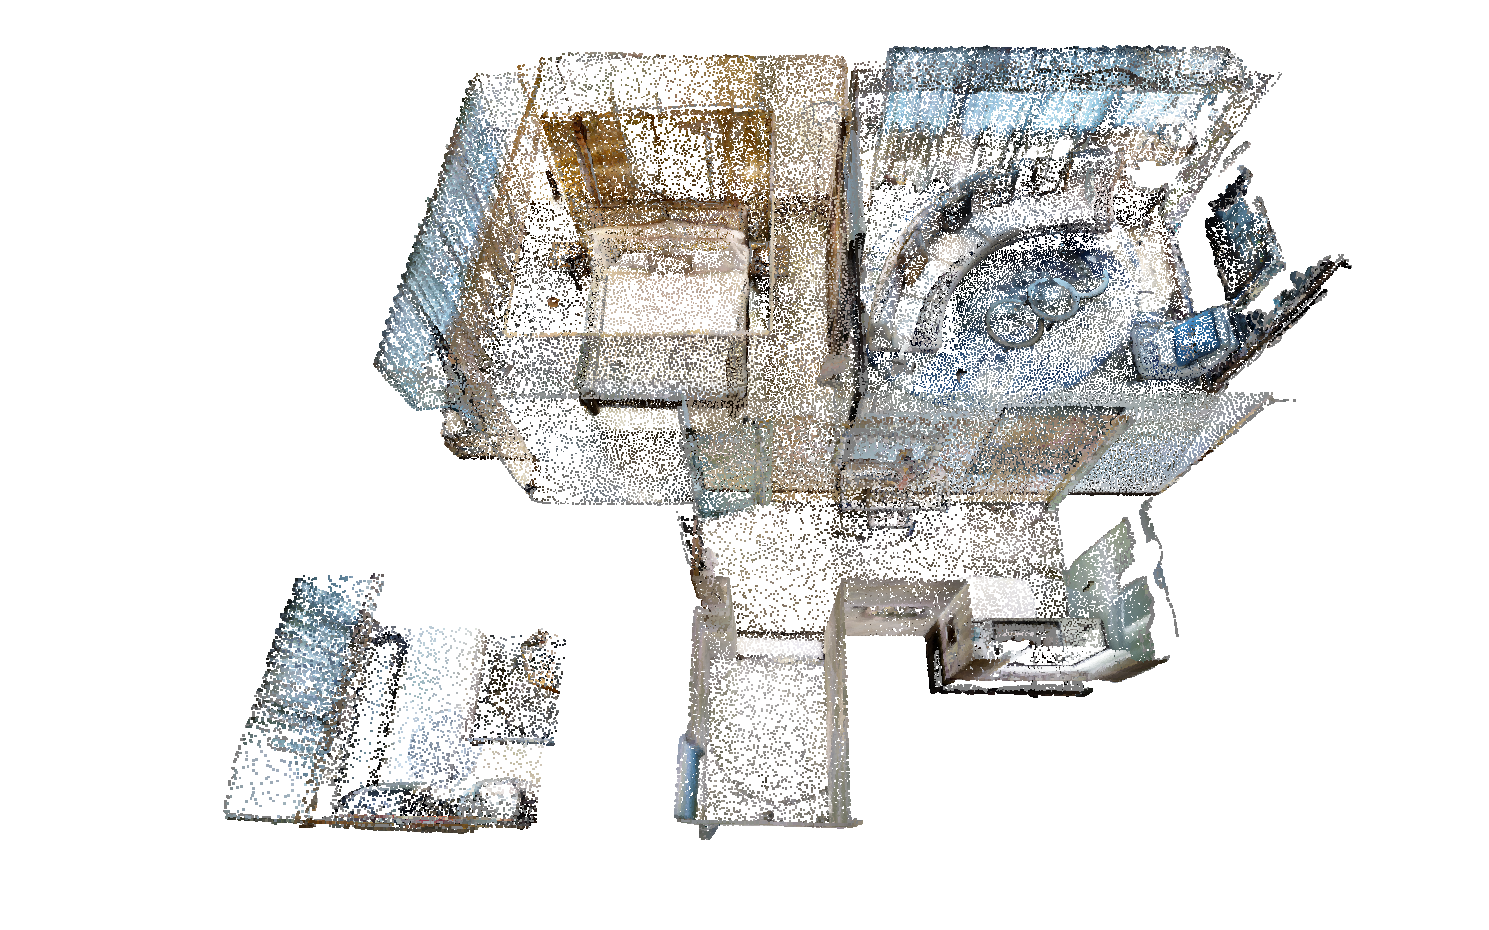
\includegraphics[width=\textwidth]{ply_log-model_1bG-gsbb_3B1-bs25-lr1-ds_30-xyz_midnorm_block-color_1norm-nxnynz-12800-mat_1083/17DRP5sb8fy_0_25_a946/raw00.png}
	\caption{colorized point cloud}
	\end{subfigure}
	\begin{subfigure}[h]{0.49\textwidth}
	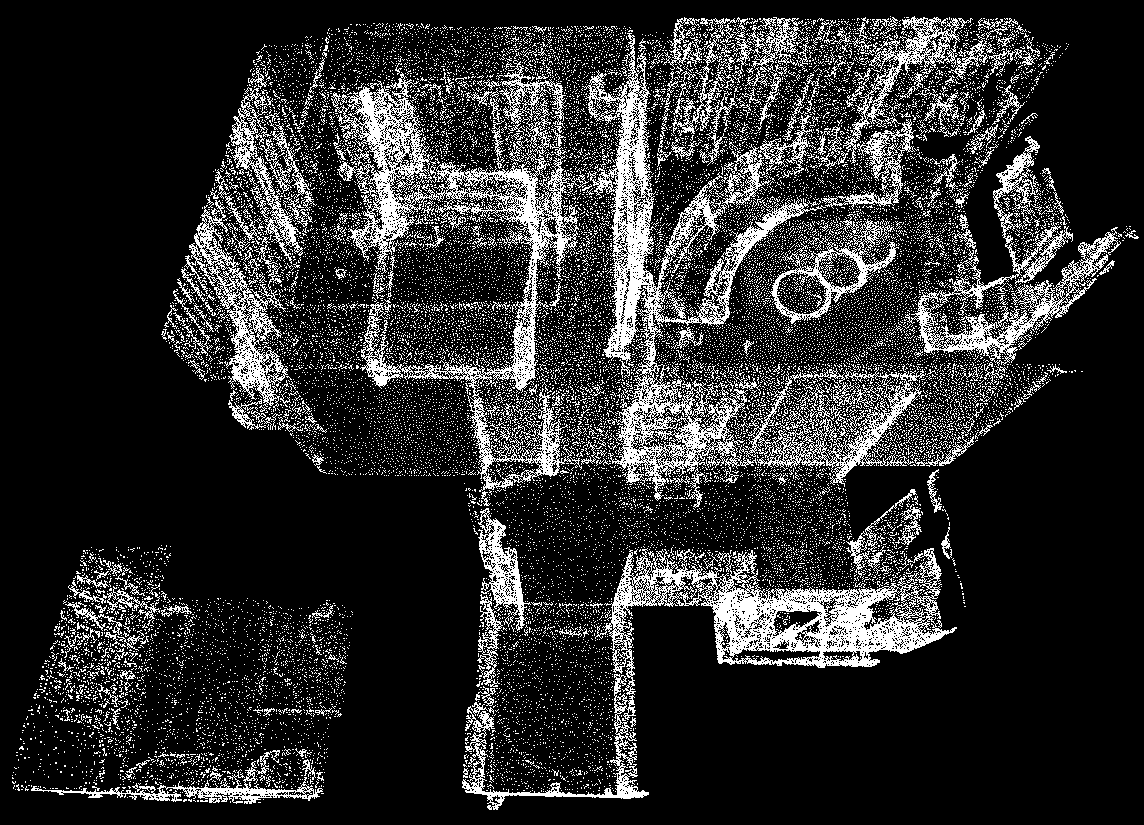
\includegraphics[width=\textwidth]{ply_log-model_1bG-gsbb_3B1-bs25-lr1-ds_30-xyz_midnorm_block-color_1norm-nxnynz-12800-mat_1083/17DRP5sb8fy_0_25_a946/xyz00.png}
	\caption{raw point cloud}
	\end{subfigure}
	\begin{subfigure}[h]{0.5\textwidth}
		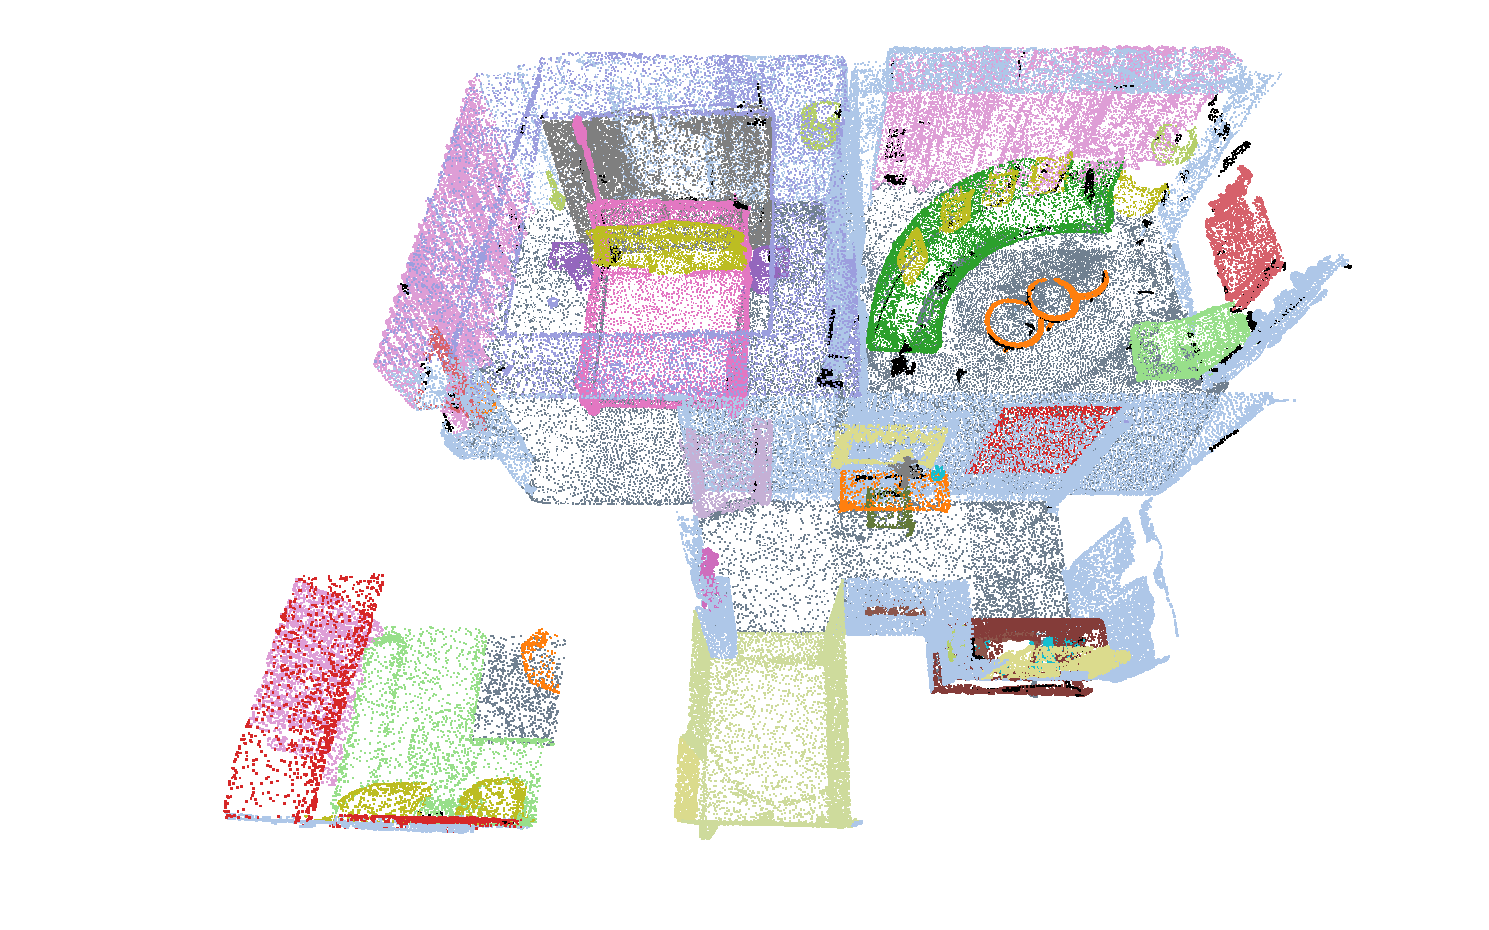
\includegraphics[width=\textwidth]{ply_log-model_1bG-gsbb_3B1-bs25-lr1-ds_30-xyz_midnorm_block-color_1norm-nxnynz-12800-mat_1083/17DRP5sb8fy_0_25_a946/gt00.png}
		\caption{gt}
	\end{subfigure}
	\begin{subfigure}[h]{0.49\textwidth}
		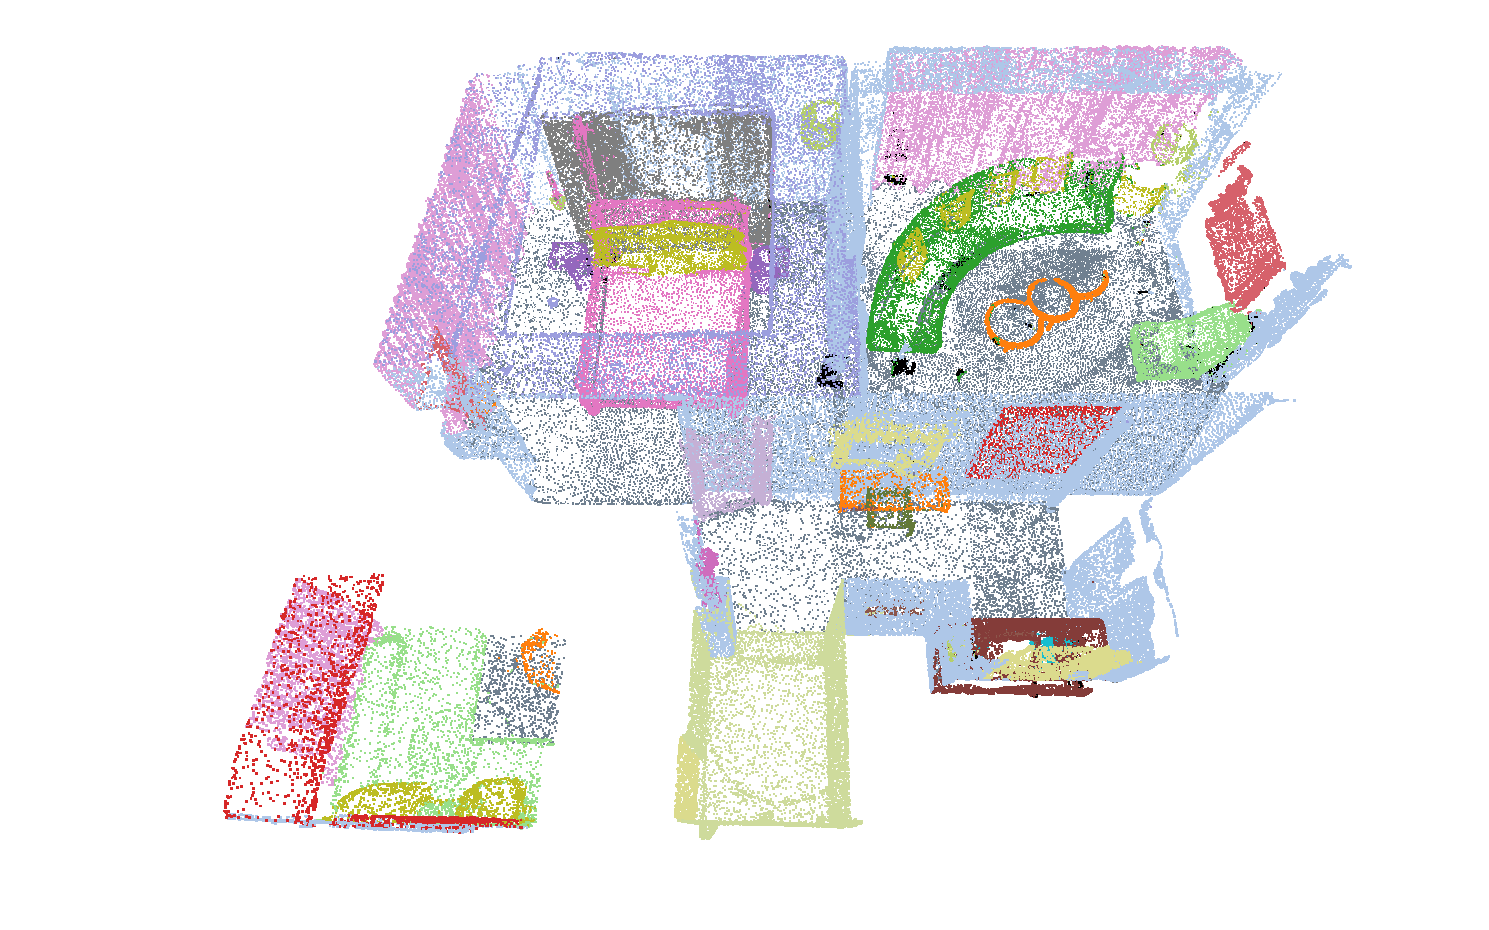
\includegraphics[width=\textwidth]{ply_log-model_1bG-gsbb_3B1-bs25-lr1-ds_30-xyz_midnorm_block-color_1norm-nxnynz-12800-mat_1083/17DRP5sb8fy_0_25_a946/pred00.png}	
		\caption{pred}
	\end{subfigure}
	\begin{subfigure}[h]{0.5\textwidth}
		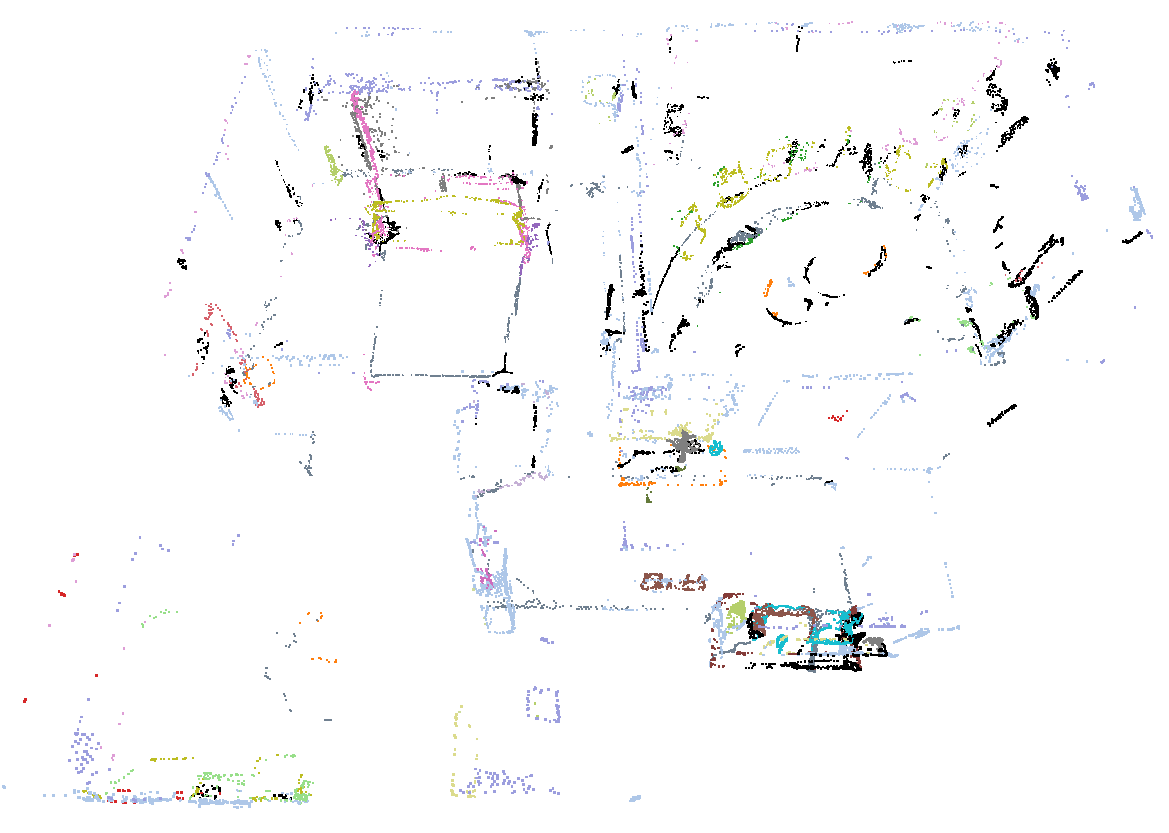
\includegraphics[width=\textwidth]{ply_log-model_1bG-gsbb_3B1-bs25-lr1-ds_30-xyz_midnorm_block-color_1norm-nxnynz-12800-mat_1083/17DRP5sb8fy_0_25_a946/err00.png}
		\caption{err}
	\end{subfigure}
	\caption{17DRP5sb8fy\_0\_25\_a946}
\end{figure}

\subsubsection{bad: 18737,eval 0.071}
model: 1bG \par
sampling \& grouping: stride\_0d1\_step\_0d1\_bmap\_nh5\_12800\_1d6\_2\_fmn3-512\_64\_24-48\_16\_12-0d2\_0d6\_1d2-0d2\_0d6\_1d2 \par
batch size: 25 \par
learning rate: 0.001000 \par
decay\_epoch\_step: 50 \par
epoch 0 train IsShuffleIdx: True  \par
epoch 0 train IsShuffleIdx: True  \par
matterport3d  \par
feed\_data\_elements:['xyz\_midnorm\_block', 'color\_1norm', 'nxnynz'] \par 
feed\_label\_elements:['label\_category', 'label\_instance']  \par
train data shape: [18737 12800     9]    \par
test data shape: [ 4172 12800     9] \par

\begin{figure}[H]
	\centering
	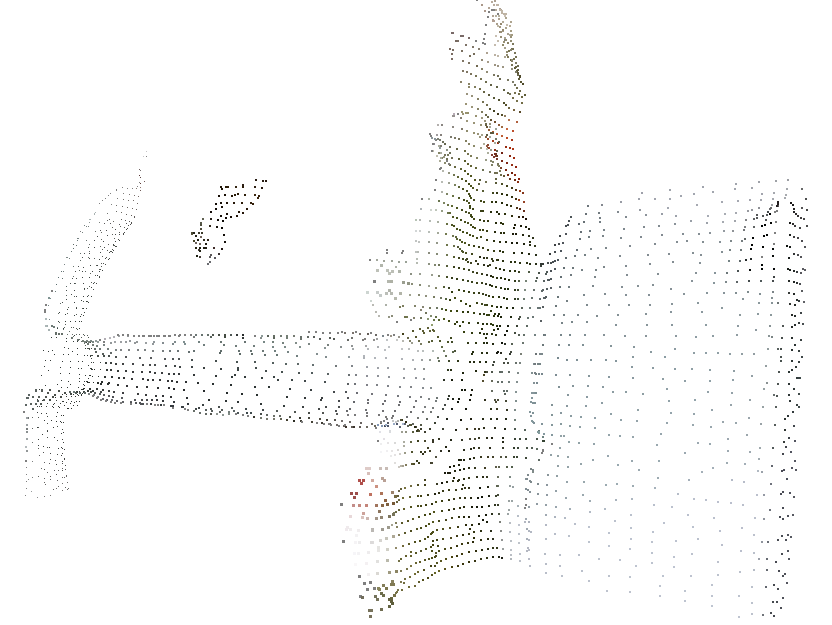
\includegraphics[width=0.49\textwidth]{ply_log-model_1bG-gsbb_3B1-bs25-lr1-ds_50-Sf_Y-xyz_midnorm_block-color_1norm-nxnynz-12800-mat_18737/qoi_r1Q_r47_rPc_rqf_2_3_raw00.png}
	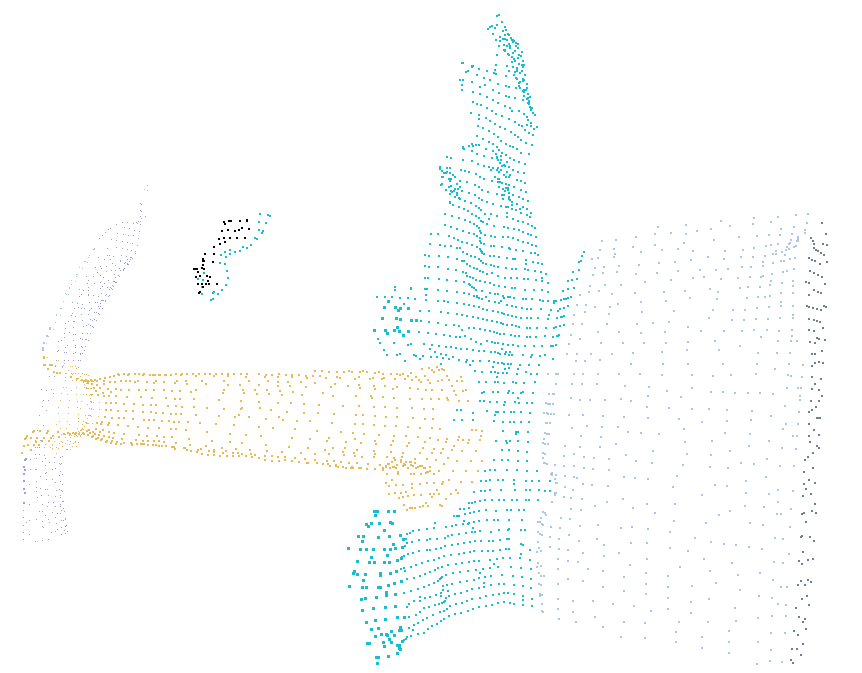
\includegraphics[width=0.49\textwidth]{ply_log-model_1bG-gsbb_3B1-bs25-lr1-ds_50-Sf_Y-xyz_midnorm_block-color_1norm-nxnynz-12800-mat_18737/qoi_r1Q_r47_rPc_rqf_2_3_gt00.png}
	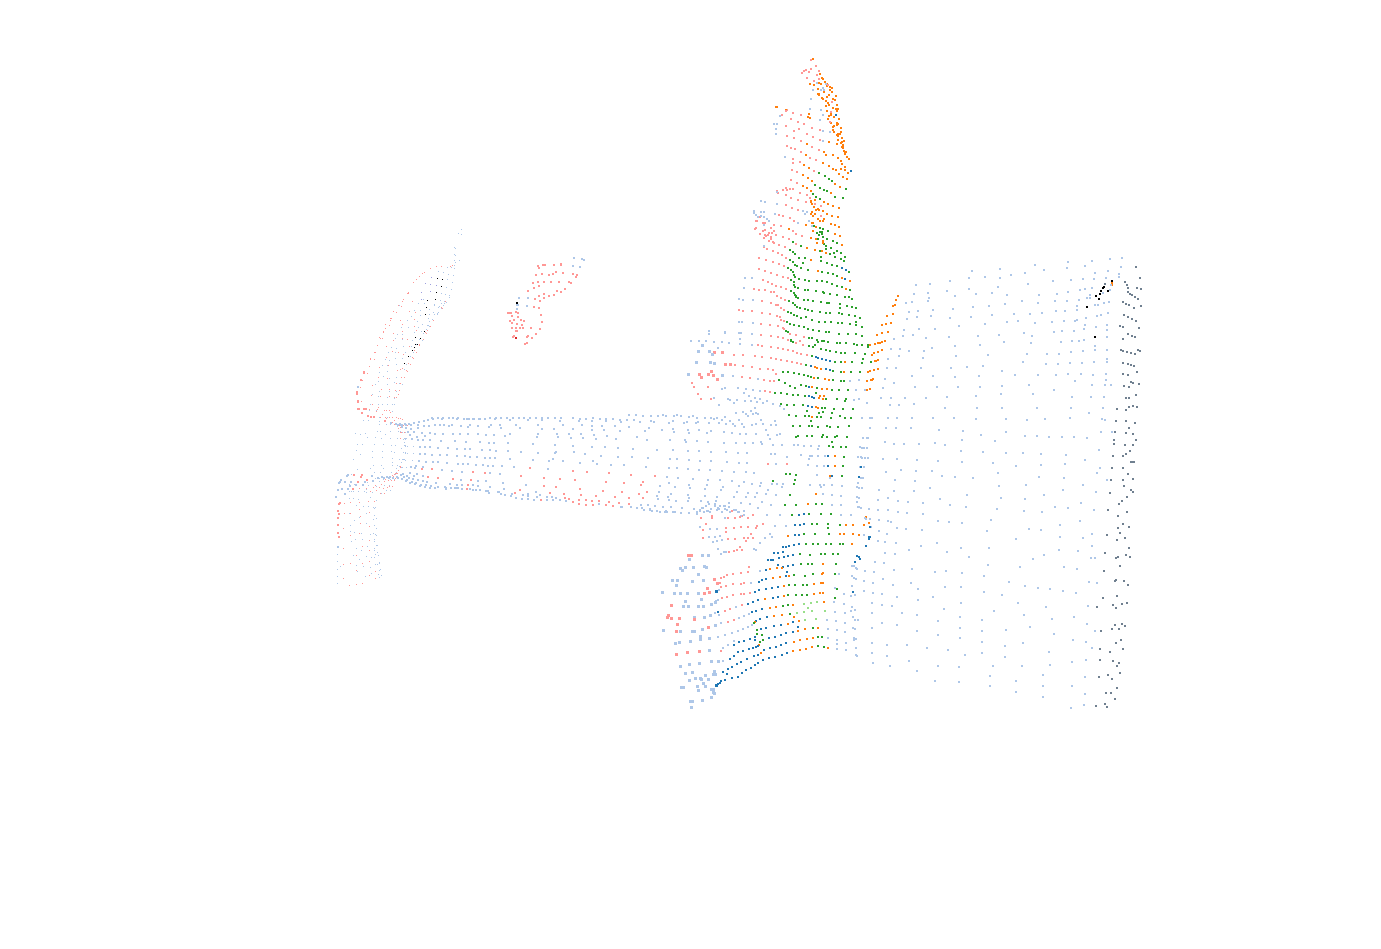
\includegraphics[width=0.49\textwidth]{ply_log-model_1bG-gsbb_3B1-bs25-lr1-ds_50-Sf_Y-xyz_midnorm_block-color_1norm-nxnynz-12800-mat_18737/qoi_r1Q_r47_rPc_rqf_2_3_pred00.png}
	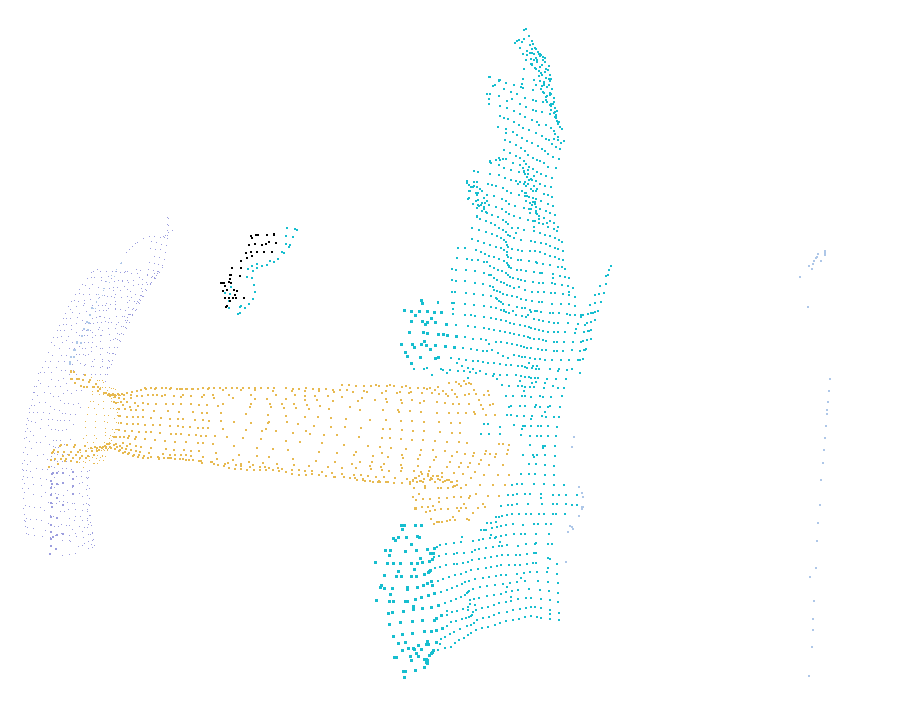
\includegraphics[width=0.49\textwidth]{ply_log-model_1bG-gsbb_3B1-bs25-lr1-ds_50-Sf_Y-xyz_midnorm_block-color_1norm-nxnynz-12800-mat_18737/qoi_r1Q_r47_rPc_rqf_2_3_a0d071_err00.png}
	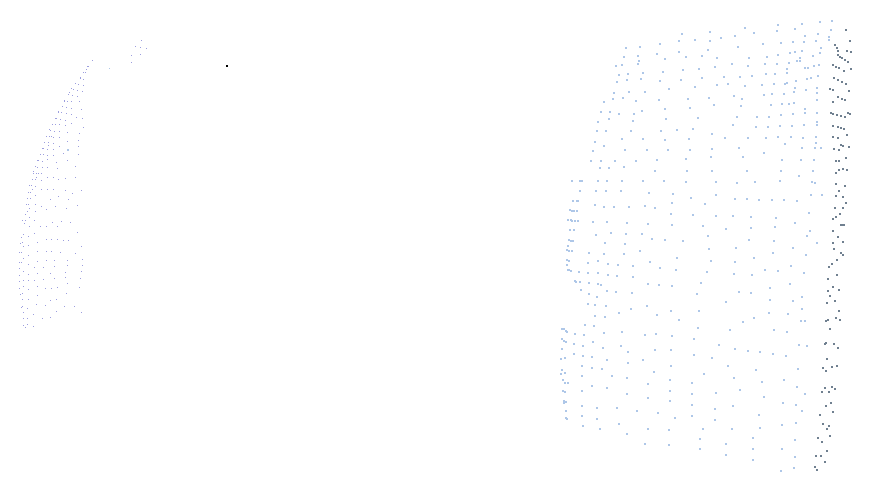
\includegraphics[width=0.49\textwidth]{ply_log-model_1bG-gsbb_3B1-bs25-lr1-ds_50-Sf_Y-xyz_midnorm_block-color_1norm-nxnynz-12800-mat_18737/qoi_r1Q_r47_rPc_rqf_2_3_a0d071_crt00.png}
	\caption{qoi\_r1Q\_r47\_rPc\_rqf\_2\_3\_a0d071 (raw,gt,pred,err,crt)}
\end{figure}


\subsection{point++}
\subsubsection{scannet seg}

\begin{center}
	\centering \def\arraystretch{1.5} \small
	\begin{tabular}{|p{1.5cm} | p{2cm} | p{3.5cm} || p{5cm}|} 
		\hline
		\multicolumn{4}{|c|}{each room as a block, total 40 block}\\
		\hline
		batch size\par batch num & lr\par ds & data elements & epoch-point ac-class ac \par train/eval/eval whole scene \\
		\hline
		30/40 & 0.001 & xyzmid & 200-0.675/0.757-0.54/0.799-0.52\\
		\hline
		25 & 0.001 & xyzmid & 200-0.689/0.787-0.556/0.815-0.517i\\
		\hline
	\end{tabular}
\end{center}

\end{document}